% Created 2015-04-26 dom 16:08
\documentclass[xcolor={usenames,svgnames,dvipsnames}]{beamer}
\usepackage[utf8]{inputenc}
\usepackage[T1]{fontenc}
\usepackage{fixltx2e}
\usepackage{graphicx}
\usepackage{longtable}
\usepackage{float}
\usepackage{wrapfig}
\usepackage{rotating}
\usepackage[normalem]{ulem}
\usepackage{amsmath}
\usepackage{textcomp}
\usepackage{marvosym}
\usepackage{wasysym}
\usepackage{amssymb}
\usepackage{hyperref}
\tolerance=1000
\usepackage{color}
\usepackage{listings}
\usecolortheme{rose}
\setbeamercolor{alerted text}{fg=Blue}
\setbeamerfont{alerted text}{series=\bfseries}
\setbeamercolor{block title}{bg=structure.fg!20!bg!50!bg}
\setbeamercolor{block body}{use=block title,bg=block title.bg}
\setbeamertemplate{navigation symbols}{}
\AtBeginSubsection[]{\begin{frame}[plain]\tableofcontents[currentsubsection,sectionstyle=show/shaded,subsectionstyle=show/shaded/hide]\end{frame}}
\lstset{keywordstyle=\color{blue}, commentstyle=\color{gray!90}, basicstyle=\ttfamily\small, columns=fullflexible, breaklines=true,linewidth=\textwidth, backgroundcolor=\color{gray!23}, basewidth={0.5em,0.4em}, literate={á}{{\'a}}1 {ñ}{{\~n}}1 {é}{{\'e}}1 {ó}{{\'o}}1 {º}{{\textordmasculine}}1}
\usepackage{mathpazo}
\hypersetup{colorlinks=true, linkcolor=Blue, urlcolor=Blue}
\usepackage{fancyvrb}
\DefineVerbatimEnvironment{verbatim}{Verbatim}{fontsize=\tiny, formatcom = {\color{black!70}}}
\usetheme{Goettingen}
\usefonttheme{serif}
\author{Oscar Perpiñán Lamigueiro \\ \url{http://oscarperpinan.github.io}}
\date{}
\title{Introducción a R}
\hypersetup{
  pdfkeywords={},
  pdfsubject={},
  pdfcreator={Emacs 24.4.1 (Org mode 8.2.7c)}}
\begin{document}

\maketitle

\section{Introducción}
\label{sec-1}
\subsection{¿Qué es \texttt{R}?}
\label{sec-1-1}
\begin{frame}[fragile,label=sec-1-1-1]{¿Qué es \texttt{R}?}
 Es un entorno de programación orientado al cálculo, manipulación de datos, y representación gráfica, publicado como software libre con licencia GNU-GPL.
\begin{center}
\url{http://www.R-project.org} 
\end{center}
\end{frame}

\begin{frame}[fragile,label=sec-1-1-2]{Para instalar \texttt{R}}
 \begin{itemize}
\item Windows: \url{http://cran.es.r-project.org/bin/windows/base/}
\item Mac: \url{http://cran.es.r-project.org/bin/macosx/}
\item Linux: \url{http://cran.es.r-project.org/bin/linux/}
\end{itemize}
\end{frame}

\begin{frame}[label=sec-1-1-3]{Interfaces para R}
\begin{itemize}
\item En mi opinión, la mejor interfaz para R es \href{http://ess.r-project.org/}{ESS} con \href{http://www.gnu.org/software/emacs/}{Emacs}.
\item Para los que prefieren una interfaz gráfica es recomendable \href{http://www.rstudio.com/ide/}{RStudio}:
\begin{itemize}
\item Instalador: \url{http://www.rstudio.com/ide/download/desktop}
\item Introducción: \url{http://www.rstudio.com/ide/docs/using/source}
\end{itemize}
\end{itemize}
\end{frame}



\begin{frame}[label=sec-1-1-4]{R está muy bien documentado}
\begin{itemize}
\item \href{http://cran.r-project.org/manuals.html}{Manuales Oficiales}

\begin{itemize}
\item \href{http://cran.r-project.org/doc/manuals/r-release/R-intro.html}{Introduction to R}

\item \href{http://cran.r-project.org/doc/manuals/r-release/R-data.html}{R Data Import/Export}

\item \href{http://cran.r-project.org/doc/manuals/r-release/R-admin.html}{R Installation and Administration}

\item \href{http://cran.r-project.org/doc/manuals/r-release/R-exts.html}{Writing R Extensions}

\item \href{http://cran.r-project.org/doc/manuals/r-release/R-lang.html}{R language definition}

\item \href{http://cran.r-project.org/doc/manuals/r-release/R-ints.html}{R Internals}
\end{itemize}

\item \href{http://cran.r-project.org/other-docs.html}{Manuales externos}
\end{itemize}
\end{frame}

\begin{frame}[label=sec-1-1-5]{Otros recursos de información}
\begin{itemize}
\item \href{http://www.r-project.org/mail.html}{Listas de correo} (sin olvidar respetar \href{http://www.r-project.org/posting-guide.html}{estos consejos})
\begin{itemize}
\item Generales: R-announce, R-help, R-devel
\item Special Interest Group (SIG) mailing lists
\end{itemize}
\item \href{http://www.r-bloggers.com}{R-bloggers}
\item \href{http://stackoverflow.com/questions/tagged/r}{stackoverflow}
\end{itemize}
\end{frame}

\begin{frame}[label=sec-1-1-6]{R es un proyecto colaborativo}
\begin{itemize}
\item Una de las grandes riquezas de R es la cantidad de paquetes (más
de 6500 actualmente) que amplían sus funcionalidades.
\item La lista completa está en \url{http://cran.es.r-project.org/web/packages/}.
\item Las CRAN Task Views agrupan por temáticas:
\url{http://cran.r-project.org/web/views/}
\end{itemize}
\end{frame}

\begin{frame}[fragile,label=sec-1-1-7]{Más de 6000 paquetes disponibles}
 \begin{itemize}
\item Algunos vienen instalados y se cargan al empezar:
\end{itemize}
\lstset{language=R,label= ,caption= ,numbers=none}
\begin{lstlisting}
  sessionInfo()
\end{lstlisting}
\end{frame}
\begin{frame}[fragile,label=sec-1-1-8]{Más de 6000 paquetes disponibles}
 \begin{itemize}
\item Otros vienen instalados pero hay que cargarlos:
\end{itemize}
\lstset{language=R,label= ,caption= ,numbers=none}
\begin{lstlisting}
  library(lattice)
  packageVersion('lattice')
\end{lstlisting}
\lstset{language=R,label= ,caption= ,numbers=none}
\begin{lstlisting}
  packageDescription('lattice')
\end{lstlisting}
\end{frame}

\begin{frame}[fragile,label=sec-1-1-9]{Más de 6000 paquetes disponibles}
 \begin{itemize}
\item Otros hay que instalarlos y después cargarlos:
\end{itemize}
\lstset{language=R,label= ,caption= ,numbers=none}
\begin{lstlisting}
  install.packages('data.table')
  library('data.table')
  packageDescription('data.table')
\end{lstlisting}
\end{frame}


\subsection{Guía para usar el curso}
\label{sec-1-2}

\begin{frame}[plain,label=sec-1-2-1]{Interfaz gráfica: RStudio}
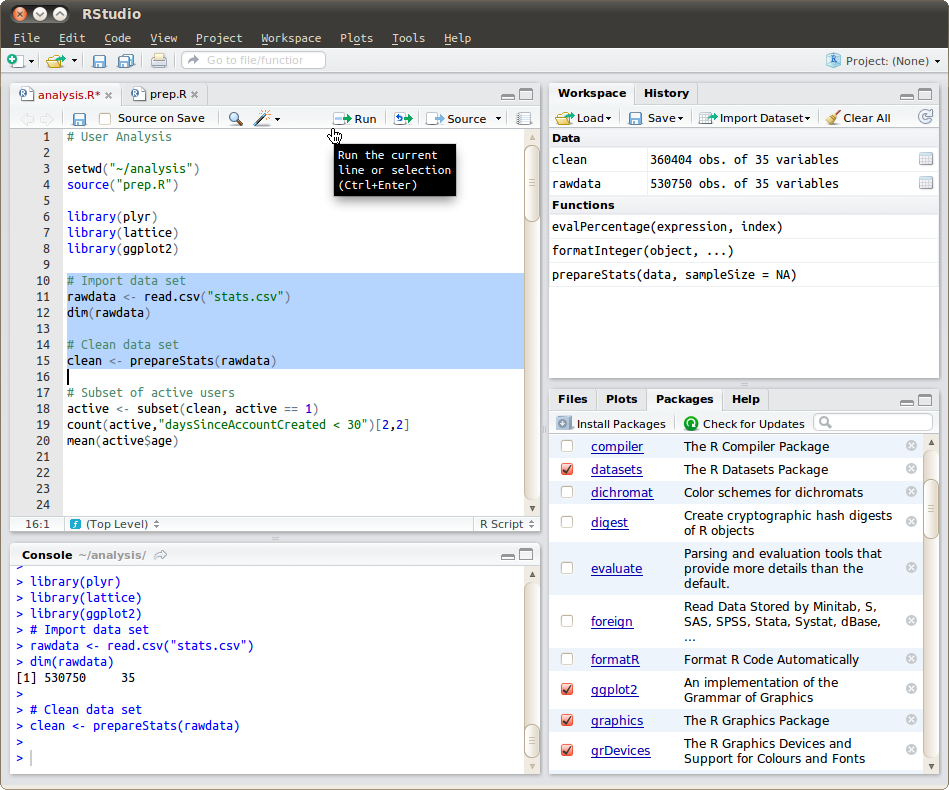
\includegraphics[width=1.05\textwidth]{figs/rstudio-ubuntu.png}
\end{frame}

\begin{frame}[fragile,label=sec-1-2-2]{Interfaz gráfica: RStudio}
 \begin{itemize}
\item La consola de R es el área en la que se ejecuta código (\texttt{Ctrl + 2})
\begin{itemize}
\item Indica con \texttt{>} que está listo para aceptar comandos.
\item Indica con \texttt{+} que está a la espera de completar comando (salir con \texttt{Esc}).
\item Permite recuperar comandos antiguos con flechas arriba y abajo.
\end{itemize}
\item El área de código es donde se edita y almacena código (\texttt{Ctrl + 1})
\begin{itemize}
\item Escribir (y grabar) en área de código y enviar a consola (\texttt{Ctrl + Enter})
\item Permite completar comandos con \texttt{TAB}
\end{itemize}
\item Para la asignación \texttt{<-} usar \texttt{Alt + -}
\end{itemize}
\end{frame}

\begin{frame}[fragile,label=sec-1-2-3]{Material}
 \begin{itemize}
\item Primero obtenemos una copia local del repositorio. Opciones:

\begin{itemize}
\item Descargando el repositorio en formato \href{https://github.com/oscarperpinan/intro/archive/master.zip}{ZIP}: descomprímelo en una ruta sencilla (por ejemplo, \texttt{C:\textbackslash{}cursoR\textbackslash{}} o \texttt{/home/miusuario/cursoR/}).

\item Usando \texttt{git}:
\end{itemize}
\end{itemize}
\lstset{language=sh,label= ,caption= ,numbers=none}
\begin{lstlisting}
git clone git://github.com/oscarperpinan/intro.git
\end{lstlisting}
\end{frame}

\begin{frame}[fragile,label=sec-1-2-4]{Material}
 \begin{itemize}
\item Todo el código del curso asume que la ruta de trabajo coincide con la carpeta local: definimos la ruta de trabajo con \texttt{setwd}
\end{itemize}
\lstset{language=R,label= ,caption= ,numbers=none}
\begin{lstlisting}
setwd('/ruta/de/copia/local/del/repositorio/')
\end{lstlisting}

\begin{itemize}
\item Comprobamos que todo ha ido bien. El resultado de la siguiente instrucción debe ser la estructura de carpetas y ficheros del repositorio:
\end{itemize}
\lstset{language=R,label= ,caption= ,numbers=none}
\begin{lstlisting}
dir()
\end{lstlisting}
\end{frame}

\begin{frame}[fragile,label=sec-1-2-5]{Material}
 \begin{itemize}
\item Finalmente hay que instalar los paquetes que se emplean a lo largo del curso. Algunos ya vendrán instalados con tu distribución de R por ser paquetes recomendados. En la siguiente instrucción usamos el \emph{CRAN mirror} de la Oficina de Software Libre (CIXUG).
\end{itemize}
\lstset{language=R,label= ,caption= ,numbers=none}
\begin{lstlisting}
install.packages(c('lattice', 'latticeExtra',
                   'RColorBrewer',
                   'zoo',
                   'reshape2', 'ggplot2'),
                 repos = 'http://ftp.cixug.es/CRAN')
\end{lstlisting}
\end{frame}

\begin{frame}[label=sec-1-2-6]{Bloc de Notas}
\begin{itemize}
\item Usaremos un bloc de notas colaborativo para escribir código juntos y resolver dudas. Está accesible en: \url{https://etsidifv.titanpad.com/r-ice-upm}

\item La clave será comunicada al inicio de las clases.
\end{itemize}
\end{frame}

\section{Objetos en R}
\label{sec-2}

\begin{frame}[fragile,label=sec-2-0-1]{Objetos en R}
 \begin{itemize}
\item Existen varios objetos en R:
\begin{itemize}
\item Vectores
\item Listas
\item Funciones
\item \ldots{}
\end{itemize}
\item A partir de estos objetos se definen varias clases:
\begin{itemize}
\item \texttt{matrix}
\item \texttt{data.frame}
\item \texttt{factor}
\item \texttt{Date}, \texttt{POSIXct}
\item \ldots{}
\end{itemize}
\end{itemize}
\end{frame}

\subsection{Vectores}
\label{sec-2-1}

\begin{frame}[fragile,label=sec-2-1-1]{Primeros pasos}
 \lstset{language=R,label= ,caption= ,numbers=none}
\begin{lstlisting}
x <- 1:5
x
\end{lstlisting}

\begin{verbatim}
[1] 1 2 3 4 5
\end{verbatim}

\lstset{language=R,label= ,caption= ,numbers=none}
\begin{lstlisting}
length(x)
\end{lstlisting}

\begin{verbatim}
[1] 5
\end{verbatim}

\lstset{language=R,label= ,caption= ,numbers=none}
\begin{lstlisting}
class(x)
\end{lstlisting}

\begin{verbatim}
[1] "integer"
\end{verbatim}
\end{frame}


\begin{frame}[fragile,label=sec-2-1-2]{Generar vectores con \texttt{seq}}
 \lstset{language=R,label= ,caption= ,numbers=none}
\begin{lstlisting}
x1 <- seq(1, 100, by=2)
x1
\end{lstlisting}

\begin{verbatim}
 [1]  1  3  5  7  9 11 13 15 17 19 21 23 25 27 29 31 33 35 37 39 41 43 45 47 49
[26] 51 53 55 57 59 61 63 65 67 69 71 73 75 77 79 81 83 85 87 89 91 93 95 97 99
\end{verbatim}

\lstset{language=R,label= ,caption= ,numbers=none}
\begin{lstlisting}
seq(1, 100, length=10)
\end{lstlisting}

\begin{verbatim}
[1]   1  12  23  34  45  56  67  78  89 100
\end{verbatim}
\end{frame}


\begin{frame}[fragile,label=sec-2-1-3]{Unir vectores con \texttt{c}}
 \lstset{language=R,label= ,caption= ,numbers=none}
\begin{lstlisting}
x <- c(1, 2, 3)
x
\end{lstlisting}

\begin{verbatim}
[1] 1 2 3
\end{verbatim}

\lstset{language=R,label= ,caption= ,numbers=none}
\begin{lstlisting}
x <- seq(1, 100, length=10)
y <- seq(2, 100, length=50)
z <- c(x, y)
z
\end{lstlisting}

\begin{verbatim}
 [1]   1  12  23  34  45  56  67  78  89 100   2   4   6   8  10  12  14  16  18
[20]  20  22  24  26  28  30  32  34  36  38  40  42  44  46  48  50  52  54  56
[39]  58  60  62  64  66  68  70  72  74  76  78  80  82  84  86  88  90  92  94
[58]  96  98 100
\end{verbatim}
\end{frame}


\begin{frame}[fragile,label=sec-2-1-4]{Operaciones sencillas con vectores}
 \lstset{language=R,label= ,caption= ,numbers=none}
\begin{lstlisting}
  x <- 1:5
  x + 1
\end{lstlisting}

\begin{verbatim}
[1] 2 3 4 5 6
\end{verbatim}

\lstset{language=R,label= ,caption= ,numbers=none}
\begin{lstlisting}
  x^2
\end{lstlisting}

\begin{verbatim}
[1]  1  4  9 16 25
\end{verbatim}

\lstset{language=R,label= ,caption= ,numbers=none}
\begin{lstlisting}
  y <- 1:10
  x + y
\end{lstlisting}

\begin{verbatim}
[1]  2  4  6  8 10  7  9 11 13 15
\end{verbatim}

\lstset{language=R,label= ,caption= ,numbers=none}
\begin{lstlisting}
  x * y
\end{lstlisting}

\begin{verbatim}
[1]  1  4  9 16 25  6 14 24 36 50
\end{verbatim}

\lstset{language=R,label= ,caption= ,numbers=none}
\begin{lstlisting}
  x^2 + y^3
\end{lstlisting}

\begin{verbatim}
[1]    2   12   36   80  150  217  347  521  745 1025
\end{verbatim}
\end{frame}




\subsection{Matrices}
\label{sec-2-2}
\begin{frame}[fragile,label=sec-2-2-1]{Construir una matriz}
 \lstset{language=R,label= ,caption= ,numbers=none}
\begin{lstlisting}
  z <- 1:12
  M  <-  matrix(z, nrow=3)
  M
\end{lstlisting}

\begin{verbatim}
     [,1] [,2] [,3] [,4]
[1,]    1    4    7   10
[2,]    2    5    8   11
[3,]    3    6    9   12
\end{verbatim}

\lstset{language=R,label= ,caption= ,numbers=none}
\begin{lstlisting}
  class(M)
\end{lstlisting}

\begin{verbatim}
[1] "matrix"
\end{verbatim}

\lstset{language=R,label= ,caption= ,numbers=none}
\begin{lstlisting}
  dim(M)
\end{lstlisting}

\begin{verbatim}
[1] 3 4
\end{verbatim}

\lstset{language=R,label= ,caption= ,numbers=none}
\begin{lstlisting}
  summary(M)
\end{lstlisting}

\begin{verbatim}
      V1            V2            V3            V4      
Min.   :1.0   Min.   :4.0   Min.   :7.0   Min.   :10.0  
1st Qu.:1.5   1st Qu.:4.5   1st Qu.:7.5   1st Qu.:10.5  
Median :2.0   Median :5.0   Median :8.0   Median :11.0  
Mean   :2.0   Mean   :5.0   Mean   :8.0   Mean   :11.0  
3rd Qu.:2.5   3rd Qu.:5.5   3rd Qu.:8.5   3rd Qu.:11.5  
Max.   :3.0   Max.   :6.0   Max.   :9.0   Max.   :12.0
\end{verbatim}
\end{frame}

\begin{frame}[fragile,label=sec-2-2-2]{Matrices a partir de vectores: \texttt{rbind} y \texttt{cbind}}
 \lstset{language=R,label= ,caption= ,numbers=none}
\begin{lstlisting}
z <- y <- x <- 1:10

M <- cbind(x, y, z)
M
\end{lstlisting}

\begin{verbatim}
       x  y  z
 [1,]  1  1  1
 [2,]  2  2  2
 [3,]  3  3  3
 [4,]  4  4  4
 [5,]  5  5  5
 [6,]  6  6  6
 [7,]  7  7  7
 [8,]  8  8  8
 [9,]  9  9  9
[10,] 10 10 10
\end{verbatim}

\lstset{language=R,label= ,caption= ,numbers=none}
\begin{lstlisting}
M <- rbind(x, y, z)
M
\end{lstlisting}

\begin{verbatim}
  [,1] [,2] [,3] [,4] [,5] [,6] [,7] [,8] [,9] [,10]
x    1    2    3    4    5    6    7    8    9    10
y    1    2    3    4    5    6    7    8    9    10
z    1    2    3    4    5    6    7    8    9    10
\end{verbatim}
\end{frame}


\subsection{Listas}
\label{sec-2-3}
\begin{frame}[fragile,label=sec-2-3-1]{Para crear una lista usamos la función \texttt{list}}
 \lstset{language=R,label= ,caption= ,numbers=none}
\begin{lstlisting}
lista <- list(a=c(1,3,5),
              b=c('l', 'p', 'r', 's'),
              c=3)
lista
\end{lstlisting}

\begin{verbatim}
$a
[1] 1 3 5

$b
[1] "l" "p" "r" "s"

$c
[1] 3
\end{verbatim}

\lstset{language=R,label= ,caption= ,numbers=none}
\begin{lstlisting}
class(lista)
\end{lstlisting}

\begin{verbatim}
[1] "list"
\end{verbatim}

\lstset{language=R,label= ,caption= ,numbers=none}
\begin{lstlisting}
length(lista)
\end{lstlisting}

\begin{verbatim}
[1] 3
\end{verbatim}
\end{frame}



\subsection{Data.frame}
\label{sec-2-4}
\begin{frame}[fragile,label=sec-2-4-1]{Para crear un \texttt{data.frame}\ldots{}}
 \lstset{language=R,label= ,caption= ,numbers=none}
\begin{lstlisting}
  df <- data.frame(x = 1:5,
                   y = rnorm(10),
                   z = 0)
  df
\end{lstlisting}

\begin{verbatim}
   x             y z
1  1  0.7085460264 0
2  2  0.0009689243 0
3  3  0.8236511370 0
4  4 -0.6323987649 0
5  5 -0.4761602237 0
6  1  1.6225023028 0
7  2  0.6327747685 0
8  3 -0.6345167308 0
9  4  0.2447118937 0
10 5 -0.4219051069 0
\end{verbatim}

\lstset{language=R,label= ,caption= ,numbers=none}
\begin{lstlisting}
  length(df)
\end{lstlisting}

\begin{verbatim}
[1] 3
\end{verbatim}

\lstset{language=R,label= ,caption= ,numbers=none}
\begin{lstlisting}
  dim(df)
\end{lstlisting}

\begin{verbatim}
[1] 10  3
\end{verbatim}
\end{frame}

\begin{frame}[fragile,label=sec-2-4-2]{La regla del reciclaje}
 \lstset{language=R,label= ,caption= ,numbers=none}
\begin{lstlisting}
  year <- 2011
  month <- 1:12
  class <- c('A', 'B', 'C')
  vals <- rnorm(12)
  
  dats <- data.frame(year, month, class, vals)
  dats
\end{lstlisting}

\begin{verbatim}
   year month class       vals
1  2011     1     A -0.9546062
2  2011     2     B  0.1911350
3  2011     3     C  1.5735383
4  2011     4     A -1.6643893
5  2011     5     B  2.2768181
6  2011     6     C -0.9075860
7  2011     7     A  0.8862328
8  2011     8     B -0.2622923
9  2011     9     C  0.9058271
10 2011    10     A -1.3207733
11 2011    11     B  0.4381335
12 2011    12     C  0.9725356
\end{verbatim}
\end{frame}

\begin{frame}[fragile,label=sec-2-4-3]{La función \texttt{expand.grid}}
 \lstset{language=R,label= ,caption= ,numbers=none}
\begin{lstlisting}
  x <- y <- seq(-4*pi, 4*pi, len=200)
  df <- expand.grid(x = x, y = y)
\end{lstlisting}

\lstset{language=R,label= ,caption= ,numbers=none}
\begin{lstlisting}
  head(df)
\end{lstlisting}

\begin{verbatim}
          x         y
1 -12.56637 -12.56637
2 -12.44008 -12.56637
3 -12.31378 -12.56637
4 -12.18749 -12.56637
5 -12.06119 -12.56637
6 -11.93489 -12.56637
\end{verbatim}

\lstset{language=R,label= ,caption= ,numbers=none}
\begin{lstlisting}
  tail(df)
\end{lstlisting}

\begin{verbatim}
             x        y
39995 11.93489 12.56637
39996 12.06119 12.56637
39997 12.18749 12.56637
39998 12.31378 12.56637
39999 12.44008 12.56637
40000 12.56637 12.56637
\end{verbatim}
\end{frame}

\subsection{Funciones}
\label{sec-2-5}

\begin{frame}[fragile,label=sec-2-5-1]{Para definir una función usamos la función \texttt{function}}
 \lstset{language=R,label= ,caption= ,numbers=none}
\begin{lstlisting}
myFun <- function(x, y) x + y
myFun
\end{lstlisting}

\begin{verbatim}
function(x, y) x + y
\end{verbatim}

\lstset{language=R,label= ,caption= ,numbers=none}
\begin{lstlisting}
  class(myFun)
\end{lstlisting}

\begin{verbatim}
[1] "function"
\end{verbatim}


\lstset{language=R,label= ,caption= ,numbers=none}
\begin{lstlisting}
  myFun(3, 4)
\end{lstlisting}

\begin{verbatim}
[1] 7
\end{verbatim}
\end{frame}

\begin{frame}[fragile,label=sec-2-5-2]{Podemos construir a partir de funciones}
 \lstset{language=R,label= ,caption= ,numbers=none}
\begin{lstlisting}
foo  <-  function(x, ...){
  mx <- mean(x, ...)
  medx <- median(x, ...)
  sdx <- sd(x, ...)
  c(mx, medx, sdx)
  }
\end{lstlisting}

O en forma resumida:
\lstset{language=R,label= ,caption= ,numbers=none}
\begin{lstlisting}
foo <- function(x, ...){c(mean(x, ...), median(x, ...), sd(x, ...))}
\end{lstlisting}
\end{frame}


\begin{frame}[fragile,label=sec-2-5-3]{Y ahora usamos la función con vectores}
 \lstset{language=R,label= ,caption= ,numbers=none}
\begin{lstlisting}
foo(1:10)
\end{lstlisting}

\begin{verbatim}
[1] 5.50000 5.50000 3.02765
\end{verbatim}

\lstset{language=R,label= ,caption= ,numbers=none}
\begin{lstlisting}
foo(rnorm(1e5))
\end{lstlisting}

\begin{verbatim}
[1] 0.0019914063 0.0003635185 1.0015828274
\end{verbatim}
\end{frame}

\section{Indexado}
\label{sec-3}

\subsection{Condiciones lógicas}
\label{sec-3-1}
\begin{frame}[fragile,label=sec-3-1-1]{Condiciones simples}
 \lstset{language=R,label= ,caption= ,numbers=none}
\begin{lstlisting}
x <- seq(-1, 1, .1)
x
\end{lstlisting}

\begin{verbatim}
 [1] -1.0 -0.9 -0.8 -0.7 -0.6 -0.5 -0.4 -0.3 -0.2 -0.1  0.0  0.1  0.2  0.3  0.4
[16]  0.5  0.6  0.7  0.8  0.9  1.0
\end{verbatim}

\lstset{language=R,label= ,caption= ,numbers=none}
\begin{lstlisting}
x < 0
\end{lstlisting}

\begin{verbatim}
 [1]  TRUE  TRUE  TRUE  TRUE  TRUE  TRUE  TRUE  TRUE  TRUE  TRUE FALSE FALSE
[13] FALSE FALSE FALSE FALSE FALSE FALSE FALSE FALSE FALSE
\end{verbatim}

\lstset{language=R,label= ,caption= ,numbers=none}
\begin{lstlisting}
x >= 0
\end{lstlisting}

\begin{verbatim}
 [1] FALSE FALSE FALSE FALSE FALSE FALSE FALSE FALSE FALSE FALSE  TRUE  TRUE
[13]  TRUE  TRUE  TRUE  TRUE  TRUE  TRUE  TRUE  TRUE  TRUE
\end{verbatim}

\lstset{language=R,label= ,caption= ,numbers=none}
\begin{lstlisting}
x != 0
\end{lstlisting}

\begin{verbatim}
 [1]  TRUE  TRUE  TRUE  TRUE  TRUE  TRUE  TRUE  TRUE  TRUE  TRUE FALSE  TRUE
[13]  TRUE  TRUE  TRUE  TRUE  TRUE  TRUE  TRUE  TRUE  TRUE
\end{verbatim}
\end{frame}

\begin{frame}[fragile,label=sec-3-1-2]{Condiciones múltiples}
 \lstset{language=R,label= ,caption= ,numbers=none}
\begin{lstlisting}
cond  <-  (x > 0) & (x < .5)
cond
\end{lstlisting}

\begin{verbatim}
 [1] FALSE FALSE FALSE FALSE FALSE FALSE FALSE FALSE FALSE FALSE FALSE  TRUE
[13]  TRUE  TRUE  TRUE FALSE FALSE FALSE FALSE FALSE FALSE
\end{verbatim}

\lstset{language=R,label= ,caption= ,numbers=none}
\begin{lstlisting}
cond  <-  (x >= .5) | (x <= -.5)
cond
\end{lstlisting}

\begin{verbatim}
 [1]  TRUE  TRUE  TRUE  TRUE  TRUE  TRUE FALSE FALSE FALSE FALSE FALSE FALSE
[13] FALSE FALSE FALSE  TRUE  TRUE  TRUE  TRUE  TRUE  TRUE
\end{verbatim}
\end{frame}


\begin{frame}[fragile,label=sec-3-1-3]{Con las condiciones se pueden hacer operaciones}
 \lstset{language=R,label= ,caption= ,numbers=none}
\begin{lstlisting}
sum(cond)
\end{lstlisting}

\begin{verbatim}
[1] 12
\end{verbatim}

\lstset{language=R,label= ,caption= ,numbers=none}
\begin{lstlisting}
sum(!cond)
\end{lstlisting}

\begin{verbatim}
[1] 9
\end{verbatim}

\lstset{language=R,label= ,caption= ,numbers=none}
\begin{lstlisting}
as.numeric(cond)
\end{lstlisting}

\begin{verbatim}
[1] 1 1 1 1 1 1 0 0 0 0 0 0 0 0 0 1 1 1 1 1 1
\end{verbatim}
\end{frame}


\subsection{Vectores}
\label{sec-3-2}
\begin{frame}[fragile,label=sec-3-2-1]{Indexado numérico}
 \lstset{language=R,label= ,caption= ,numbers=none}
\begin{lstlisting}
  x <- seq(1, 100, 2)
  x
\end{lstlisting}

\begin{verbatim}
 [1]  1  3  5  7  9 11 13 15 17 19 21 23 25 27 29 31 33 35 37 39 41 43 45 47 49
[26] 51 53 55 57 59 61 63 65 67 69 71 73 75 77 79 81 83 85 87 89 91 93 95 97 99
\end{verbatim}

\lstset{language=R,label= ,caption= ,numbers=none}
\begin{lstlisting}
  x[1:5]
\end{lstlisting}

\begin{verbatim}
[1] 1 3 5 7 9
\end{verbatim}

\lstset{language=R,label= ,caption= ,numbers=none}
\begin{lstlisting}
  x[10:5]
\end{lstlisting}

\begin{verbatim}
[1] 19 17 15 13 11  9
\end{verbatim}
\end{frame}

\begin{frame}[fragile,label=sec-3-2-2]{Indexado con condiciones lógicas}
 \lstset{language=R,label= ,caption= ,numbers=none}
\begin{lstlisting}
  x == 37
\end{lstlisting}

\begin{verbatim}
 [1] FALSE FALSE FALSE FALSE FALSE FALSE FALSE FALSE FALSE FALSE FALSE FALSE
[13] FALSE FALSE FALSE FALSE FALSE FALSE  TRUE FALSE FALSE FALSE FALSE FALSE
[25] FALSE FALSE FALSE FALSE FALSE FALSE FALSE FALSE FALSE FALSE FALSE FALSE
[37] FALSE FALSE FALSE FALSE FALSE FALSE FALSE FALSE FALSE FALSE FALSE FALSE
[49] FALSE FALSE
\end{verbatim}

\lstset{language=R,label= ,caption= ,numbers=none}
\begin{lstlisting}
  x[x == 37]
\end{lstlisting}

\begin{verbatim}
[1] 37
\end{verbatim}

\lstset{language=R,label= ,caption= ,numbers=none}
\begin{lstlisting}
  x[x != 9]
\end{lstlisting}

\begin{verbatim}
 [1]  1  3  5  7 11 13 15 17 19 21 23 25 27 29 31 33 35 37 39 41 43 45 47 49 51
[26] 53 55 57 59 61 63 65 67 69 71 73 75 77 79 81 83 85 87 89 91 93 95 97 99
\end{verbatim}

\lstset{language=R,label= ,caption= ,numbers=none}
\begin{lstlisting}
  x[x > 20]
\end{lstlisting}

\begin{verbatim}
 [1] 21 23 25 27 29 31 33 35 37 39 41 43 45 47 49 51 53 55 57 59 61 63 65 67 69
[26] 71 73 75 77 79 81 83 85 87 89 91 93 95 97 99
\end{verbatim}
\end{frame}



\begin{frame}[fragile,label=sec-3-2-3]{Indexado con condiciones múltiples}
 \lstset{language=R,label= ,caption= ,numbers=none}
\begin{lstlisting}
z <- seq(-10, 10, by = .5)
z
\end{lstlisting}

\begin{verbatim}
 [1] -10.0  -9.5  -9.0  -8.5  -8.0  -7.5  -7.0  -6.5  -6.0  -5.5  -5.0  -4.5
[13]  -4.0  -3.5  -3.0  -2.5  -2.0  -1.5  -1.0  -0.5   0.0   0.5   1.0   1.5
[25]   2.0   2.5   3.0   3.5   4.0   4.5   5.0   5.5   6.0   6.5   7.0   7.5
[37]   8.0   8.5   9.0   9.5  10.0
\end{verbatim}

\lstset{language=R,label= ,caption= ,numbers=none}
\begin{lstlisting}
z[z < -5 | z > 5]
\end{lstlisting}

\begin{verbatim}
 [1] -10.0  -9.5  -9.0  -8.5  -8.0  -7.5  -7.0  -6.5  -6.0  -5.5   5.5   6.0
[13]   6.5   7.0   7.5   8.0   8.5   9.0   9.5  10.0
\end{verbatim}

\lstset{language=R,label= ,caption= ,numbers=none}
\begin{lstlisting}
cond <- (z >= 0 & z <= 5)
cond
\end{lstlisting}

\begin{verbatim}
 [1] FALSE FALSE FALSE FALSE FALSE FALSE FALSE FALSE FALSE FALSE FALSE FALSE
[13] FALSE FALSE FALSE FALSE FALSE FALSE FALSE FALSE  TRUE  TRUE  TRUE  TRUE
[25]  TRUE  TRUE  TRUE  TRUE  TRUE  TRUE  TRUE FALSE FALSE FALSE FALSE FALSE
[37] FALSE FALSE FALSE FALSE FALSE
\end{verbatim}

\lstset{language=R,label= ,caption= ,numbers=none}
\begin{lstlisting}
z[cond]
\end{lstlisting}

\begin{verbatim}
[1] 0.0 0.5 1.0 1.5 2.0 2.5 3.0 3.5 4.0 4.5 5.0
\end{verbatim}
\end{frame}

\subsection{Matrices}
\label{sec-3-3}
\begin{frame}[fragile,label=sec-3-3-1]{Indexado de matrices}
 \lstset{language=R,label= ,caption= ,numbers=none}
\begin{lstlisting}
M[1:2, ]
\end{lstlisting}

\begin{verbatim}
  [,1] [,2] [,3] [,4] [,5] [,6] [,7] [,8] [,9] [,10]
x    1    2    3    4    5    6    7    8    9    10
y    1    2    3    4    5    6    7    8    9    10
\end{verbatim}

\lstset{language=R,label= ,caption= ,numbers=none}
\begin{lstlisting}
M[1:2, 2:3]
\end{lstlisting}

\begin{verbatim}
  [,1] [,2]
x    2    3
y    2    3
\end{verbatim}

\lstset{language=R,label= ,caption= ,numbers=none}
\begin{lstlisting}
M[1, c(1, 4)]
\end{lstlisting}

\begin{verbatim}
[1] 1 4
\end{verbatim}
\end{frame}

\begin{frame}[fragile,label=sec-3-3-2]{Indexado de matrices}
 \lstset{language=R,label= ,caption= ,numbers=none}
\begin{lstlisting}
M[-1,]
\end{lstlisting}

\begin{verbatim}
  [,1] [,2] [,3] [,4] [,5] [,6] [,7] [,8] [,9] [,10]
y    1    2    3    4    5    6    7    8    9    10
z    1    2    3    4    5    6    7    8    9    10
\end{verbatim}

\lstset{language=R,label= ,caption= ,numbers=none}
\begin{lstlisting}
M[-c(1, 2),]
\end{lstlisting}

\begin{verbatim}
[1]  1  2  3  4  5  6  7  8  9 10
\end{verbatim}
\end{frame}

\subsection{Listas}
\label{sec-3-4}
\begin{frame}[fragile,label=sec-3-4-1]{Podemos acceder a los elementos\ldots{}}
 \begin{itemize}
\item Por su nombre
\end{itemize}
\lstset{language=R,label= ,caption= ,numbers=none}
\begin{lstlisting}
lista$a
\end{lstlisting}

\begin{verbatim}
[1] 1 3 5
\end{verbatim}

\begin{itemize}
\item o por su índice
\end{itemize}
\lstset{language=R,label= ,caption= ,numbers=none}
\begin{lstlisting}
  lista[1]
\end{lstlisting}

\begin{verbatim}
$a
[1] 1 3 5
\end{verbatim}

\lstset{language=R,label= ,caption= ,numbers=none}
\begin{lstlisting}
  lista[[1]]
\end{lstlisting}

\begin{verbatim}
[1] 1 3 5
\end{verbatim}
\end{frame}


\subsection{Data Frame}
\label{sec-3-5}
\begin{frame}[fragile,label=sec-3-5-1]{Podemos acceder a los elementos}
 \lstset{language=R,label= ,caption= ,numbers=none}
\begin{lstlisting}
  df <- data.frame(x = 1:5,
                   y = rnorm(10),
                   z = 0)
\end{lstlisting}

\begin{itemize}
\item Por su nombre (como una lista)
\end{itemize}
\lstset{language=R,label= ,caption= ,numbers=none}
\begin{lstlisting}
df$x
\end{lstlisting}

\begin{verbatim}
[1] 1 2 3 4 5 1 2 3 4 5
\end{verbatim}

\begin{itemize}
\item Por su índice (como una matriz)
\end{itemize}
\lstset{language=R,label= ,caption= ,numbers=none}
\begin{lstlisting}
df[1,]
\end{lstlisting}

\begin{verbatim}
  x          y z
1 1 -0.1354198 0
\end{verbatim}

\lstset{language=R,label= ,caption= ,numbers=none}
\begin{lstlisting}
df[,1]
\end{lstlisting}

\begin{verbatim}
[1] 1 2 3 4 5 1 2 3 4 5
\end{verbatim}
\end{frame}

\section{Bucles}
\label{sec-4}
\subsection{Matrices}
\label{sec-4-1}
\begin{frame}[fragile,label=sec-4-1-1]{La función \texttt{apply}}
 \lstset{language=R,label= ,caption= ,numbers=none}
\begin{lstlisting}
apply(M, 1, sum)
\end{lstlisting}

\begin{verbatim}
 x  y  z 
55 55 55
\end{verbatim}

\lstset{language=R,label= ,caption= ,numbers=none}
\begin{lstlisting}
rowSums(M)
\end{lstlisting}

\begin{verbatim}
 x  y  z 
55 55 55
\end{verbatim}

\lstset{language=R,label= ,caption= ,numbers=none}
\begin{lstlisting}
apply(M, 2, mean)
\end{lstlisting}

\begin{verbatim}
[1]  1  2  3  4  5  6  7  8  9 10
\end{verbatim}

\lstset{language=R,label= ,caption= ,numbers=none}
\begin{lstlisting}
colMeans(M)
\end{lstlisting}

\begin{verbatim}
[1]  1  2  3  4  5  6  7  8  9 10
\end{verbatim}
\end{frame}

\subsection{Listas / \texttt{data.frame}}
\label{sec-4-2}
\begin{frame}[fragile,label=sec-4-2-1]{\texttt{lapply} y \texttt{sapply}}
 \lstset{language=R,label= ,caption= ,numbers=none}
\begin{lstlisting}
lista <- list(x = 1:10,
              y = seq(0, 10, 2),
              z = rnorm(30))
lapply(lista, sum)
\end{lstlisting}

\begin{verbatim}
$x
[1] 55

$y
[1] 30

$z
[1] 2.516194
\end{verbatim}

\lstset{language=R,label= ,caption= ,numbers=none}
\begin{lstlisting}
sapply(lista, sum)
\end{lstlisting}

\begin{verbatim}
        x         y         z 
55.000000 30.000000  2.516194
\end{verbatim}
\end{frame}

\subsection{Bucles \texttt{for}}
\label{sec-4-3}
\begin{frame}[fragile,label=sec-4-3-1]{\texttt{for}}
 \begin{itemize}
\item En \texttt{R} suele usarse más la familia de funciones \texttt{*apply} con funciones vectorizadas.
\end{itemize}
\lstset{language=R,label= ,caption= ,numbers=none}
\begin{lstlisting}
for(n in c(2,5,10,20,50)) {
    x <- rnorm(n)
    cat(n,":", sum(x^2),"\n")
}
\end{lstlisting}

\begin{verbatim}
2 : 1.519747 
5 : 6.492911 
10 : 17.80714 
20 : 27.50484 
50 : 37.55957
\end{verbatim}
\end{frame}

\subsection{Condiciones con \texttt{if}, \texttt{else} e \texttt{ifelse}}
\label{sec-4-4}
\begin{frame}[fragile,label=sec-4-4-1]{\texttt{if}}
 \begin{itemize}
\item En \texttt{R} suele usarse más el indexado lógico (vectorizado).
\end{itemize}
\lstset{language=R,label= ,caption= ,numbers=none}
\begin{lstlisting}
  x <- rnorm(10)
  x2 <- numeric(length(x))
  for (i in seq_along(x2)){
      if (x[i]<0) x2[i] <- 0 else x2[i] <- 1
      }
  cbind(x, x2)
\end{lstlisting}

\begin{verbatim}
                x x2
 [1,] -0.06946282  0
 [2,]  2.21631558  1
 [3,] -1.73203394  0
 [4,]  0.51881647  1
 [5,]  1.16850807  1
 [6,] -0.83734030  0
 [7,] -1.58535710  0
 [8,] -0.30040180  0
 [9,] -0.14779841  0
[10,]  3.21988159  1
\end{verbatim}
\end{frame}

\begin{frame}[fragile,label=sec-4-4-2]{\texttt{ifelse}}
 \lstset{language=R,label= ,caption= ,numbers=none}
\begin{lstlisting}
x <- rnorm(10)
x
\end{lstlisting}

\begin{verbatim}
[1]  1.3506244  0.3312057  2.0949944  1.4803420 -0.3592188 -0.4912907
[7]  0.2853986 -1.2526219 -0.6463107 -1.8632414
\end{verbatim}

\lstset{language=R,label= ,caption= ,numbers=none}
\begin{lstlisting}
ifelse(x>0, 1, 0)
\end{lstlisting}

\begin{verbatim}
[1] 1 1 1 1 0 0 1 0 0 0
\end{verbatim}
\end{frame}
% Emacs 24.4.1 (Org mode 8.2.7c)
\end{document}